\section{Проектирование и разработка программного средства}

\subsection{Архитектура программного средства}

Процесс разработки программного обеспечения для голосового помощника для одноплатного компьютера требует внимательного подхода к проектированию, с учётом особенностей работы на ограниченных ресурсах и необходимости обеспечения масштабируемости и расширяемости. Для эффективного решения этих задач был выбран объектно-ориентированный подход, который обеспечил чёткое разделение функциональности на независимые и легко заменяемые компоненты.

Программное средство состоит из следующих основных компонентов:

\begin{itemize}
	\item {Core::VoiceAssistant} — центральный компонент, управляющий жизненным циклом голосового помощника. Он отвечает за инициализацию всех необходимых модулей и запуск основного цикла обработки команд.
	
	\item {Speach::SpeechRecognizer} — модуль распознавания речи, использующий библиотеку \textit{Vosk} и \text{PortAudio} для захвата и анализа аудиопотока с микрофона.
	
	\item {CommandManager} — отвечает за регистрацию голосовых команд и выполнение соответствующих обработчиков при их распознавании.
\end{itemize}

Взаимодействие между компонентами организовано следующим образом: \texttt{VoiceAssistant} инициализирует экземпляр \texttt{SpeechRecognizer}, а затем в бесконечном цикле получает голосовой ввод, преобразованный в текст. Полученный текст передаётся в \texttt{CommandManager}, который анализирует его и при обнаружении соответствующей команды вызывает заранее зарегистрированную функцию-обработчик. Таким образом реализована цепочка: \textbf{распознавание}~$\rightarrow$~\textbf{анализ}~$\rightarrow$~\textbf{выполнение}.

Такой подход позволяет легко расширять систему, добавляя новые голосовые команды, не затрагивая существующую логику работы помощника.

\subsection{Реализация основных модулей}

На представленном рисунке \ref{fig:main.cpp} показан исходный код на языке C++, реализующий точку входа в систему голосового помощника.
\begin{figure}[H]
	\centering
	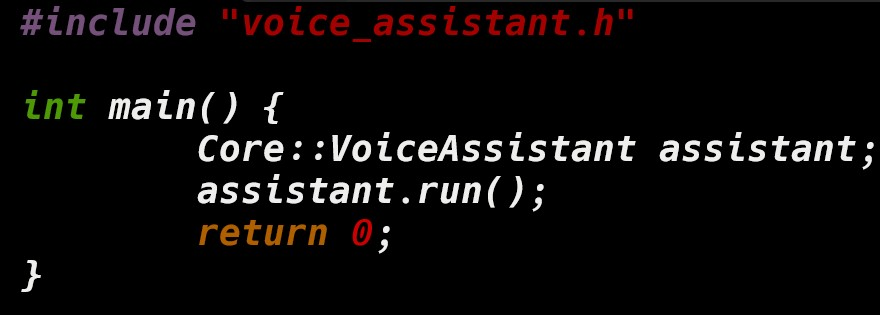
\includegraphics[scale=0.5]{main.jpg}
	\caption{Точка входа в программную систему}
	\label{fig:main.cpp}
\end{figure}

\begin{figure}[H]
	\centering
	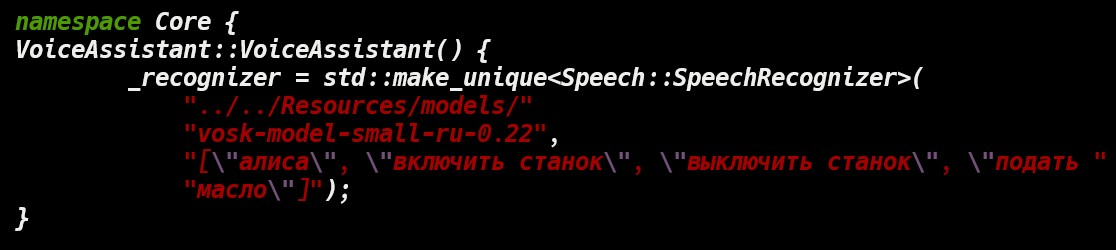
\includegraphics[scale=0.5]{constructor_VoiceAssistant.jpg}
	\caption{Конструктор VoiceAssistant}
\end{figure}

При создании объекта VoiceAssistant:
\begin{itemize}
 	\item Загружается модель распознавания речи Vosk для русского языка.

	\item Настраивается ограниченный набор фраз, которые ассистент сможет распознавать. Это повышает точность, так как система не пытается распознать произвольную речь, а ждёт только указанные команды.
\end{itemize}

\begin{figure}[H]
	\centering
	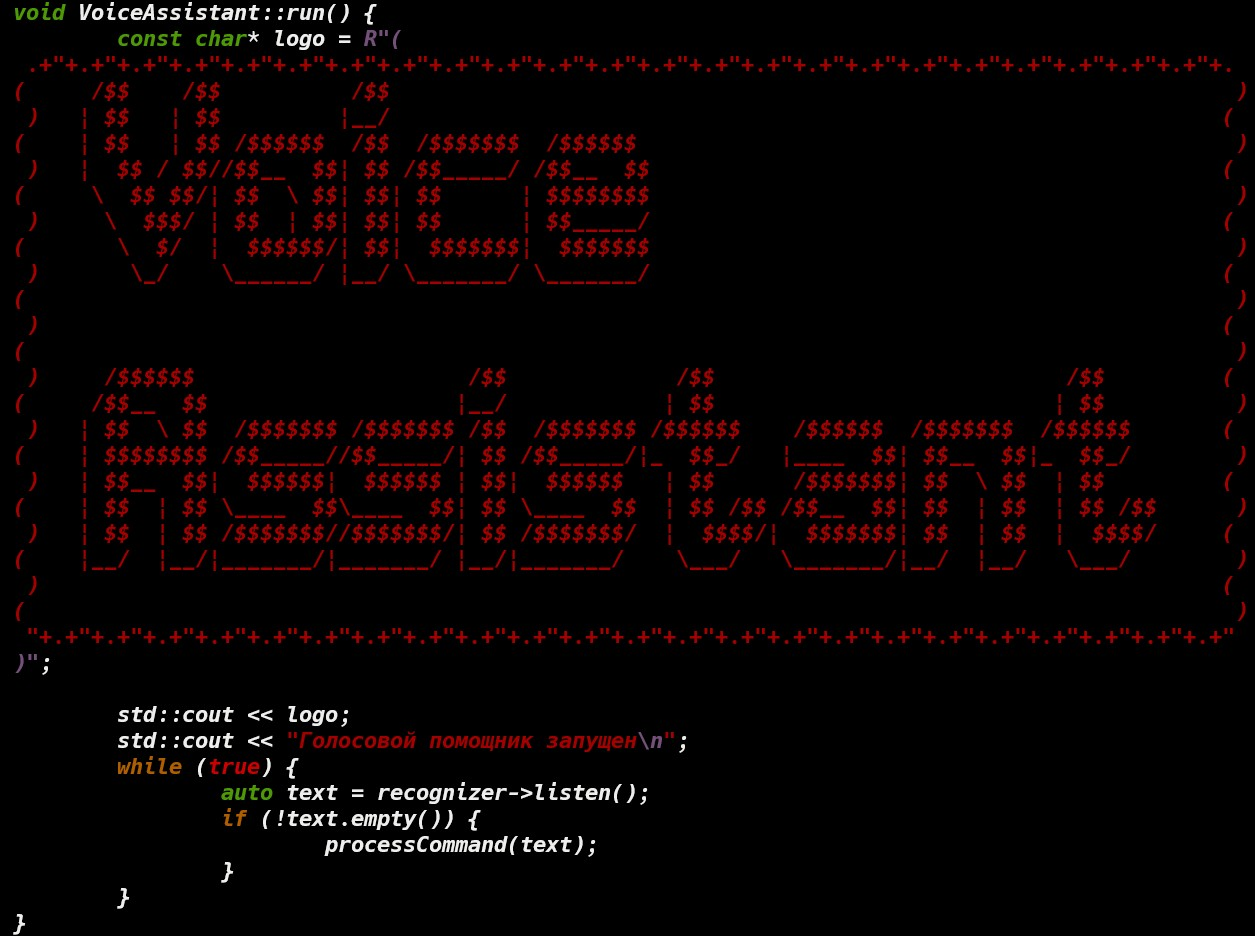
\includegraphics[scale=0.7]{run_VoiceAssistant.jpg}
	\caption{Метод run() класса VoiceAssistant}
\end{figure}

Метод VoiceAssistant::run() обеспечивает запуск и непрерывную работу голосового ассистента. В начале работы выводится ASCII-графика в виде стилизованного баннера, созданного с помощью raw-строки для удобного многострочного форматирования. Сразу после отображения логотипа программа выводит текстовое сообщение "Голосовой помощник запущен", сигнализирующее о начале работы системы. Основная функциональность реализована через бесконечный цикл, в котором непрерывно происходит захват аудиопотока через метод recognizer->listen(), преобразование звукового сигнала в текст с использованием модели распознавания речи Vosk и последующая обработка полученных команд. Распознанный текст проверяется на пустоту, и при успешном распознавании передается в метод processCommand() для выполнения соответствующих действий. Система работает в постоянном режиме ожидания голосовых команд до принудительного завершения работы программы, при этом все пустые или нераспознанные аудиофрагменты автоматически игнорируются для предотвращения ложных срабатываний. Реализация использует предобученную модель Vosk для русского языка с ограниченным набором команд, что обеспечивает высокую точность распознавания при работе с заданными фразами-триггерами. Алгоритм работы представляет собой последовательность непрерывно повторяющихся операций: захват аудиосигнала, преобразование речи в текст, валидация результата и выполнение соответствующей команды через механизм обработки голосовых инструкций.

\begin{figure}[H]
	\centering
	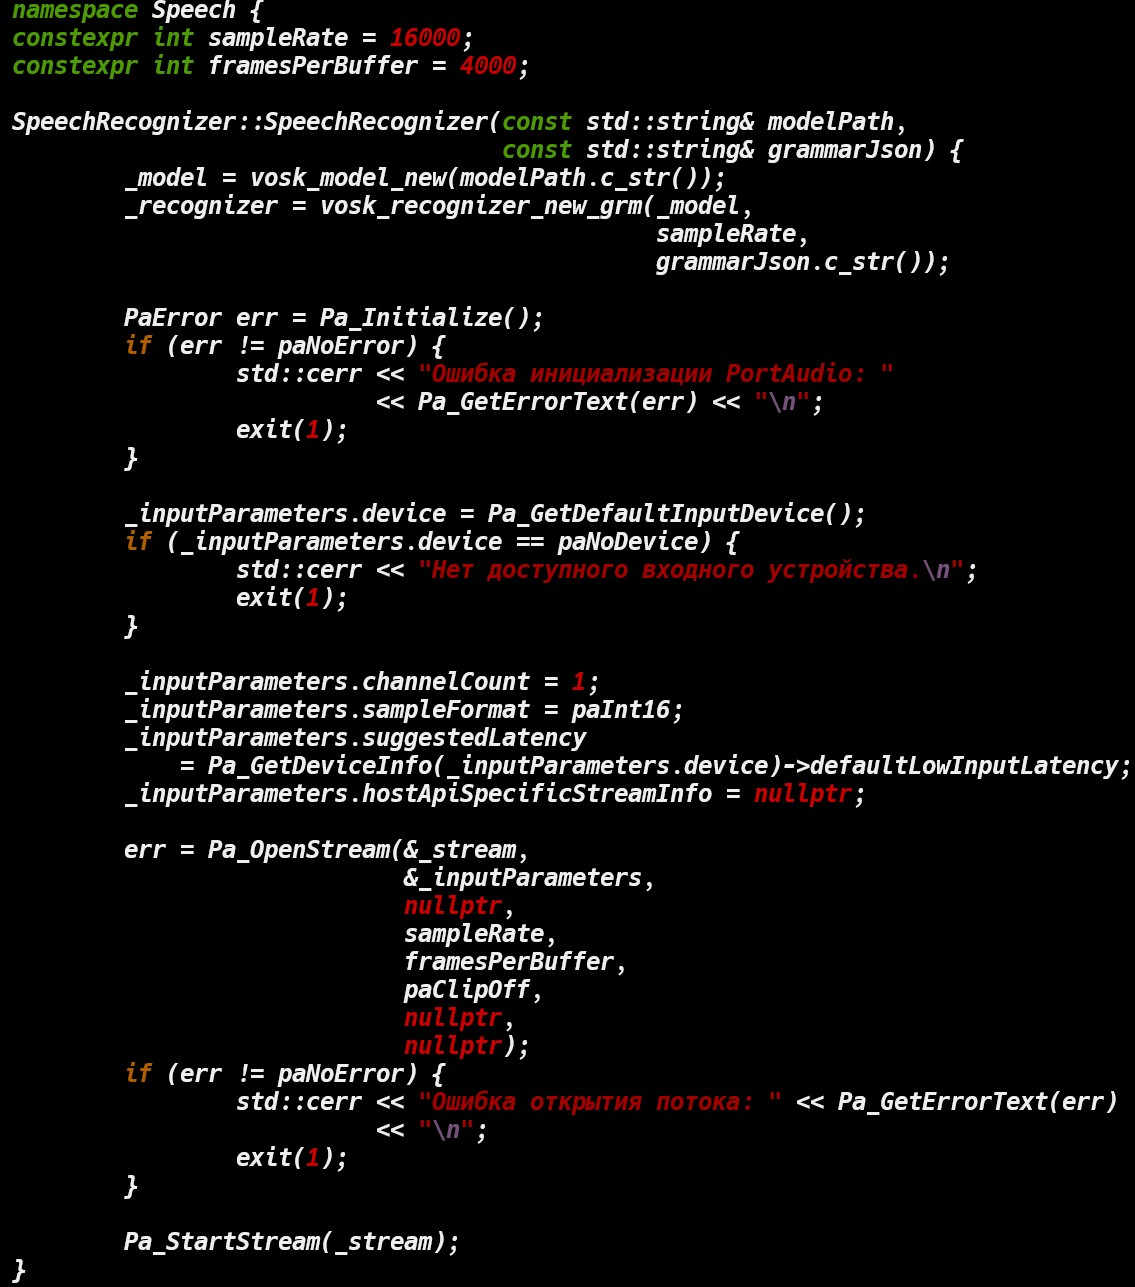
\includegraphics[scale=0.7]{constructor_SpeechRecognizer.jpg}
	\caption{Конструктор SpeechRecognizer}
\end{figure}

Конструктор класса SpeechRecognizer выполняет инициализацию системы распознавания речи, начиная с загрузки акустической модели Vosk по указанному пути. Для работы с голосовыми командами создается распознаватель с ограниченной грамматикой, заданной в JSON-формате, что позволяет системе фокусироваться только на указанных фразах-триггерах. Частота дискретизации аудиопотока фиксирована на значении 16 кГц, что является стандартом для задач распознавания речи, а размер буфера для обработки установлен в 4000 сэмплов.

Инициализация аудиовхода осуществляется через библиотеку PortAudio, где сначала проверяется наличие доступных записывающих устройств. Если микрофон обнаружен, настраиваются параметры аудиопотока: одноканальный режим (моно), 16-битный целочисленный формат данных и рекомендуемая задержка, взятая из характеристик устройства. При возникновении ошибок на любом этапе (отсутствие устройства, проблемы с открытием потока) программа аварийно завершается с выводом соответствующего сообщения. После успешной настройки аудиопоток запускается в режиме реального времени, что позволяет начать передачу аудиоданных в распознаватель Vosk для последующей обработки.

Весь процесс инициализации включает четыре ключевых этапа: создание модели распознавания, конфигурацию аудиоинтерфейса, открытие звукового потока и его активацию. Использование фиксированных параметров (частота дискретизации, размер буфера) гарантирует стабильную работу системы на оборудовании с разными характеристиками, а обработка ошибок на каждом этапе обеспечивает корректное поведение при отсутствии необходимых компонентов. Полученный экземпляр распознавателя готов к непрерывной записи и анализу аудиосигнала через вызов соответствующего метода, который будет передавать данные в модель Vosk для преобразования речи в текст согласно заданной грамматике.

\begin{figure}[H]
	\centering
	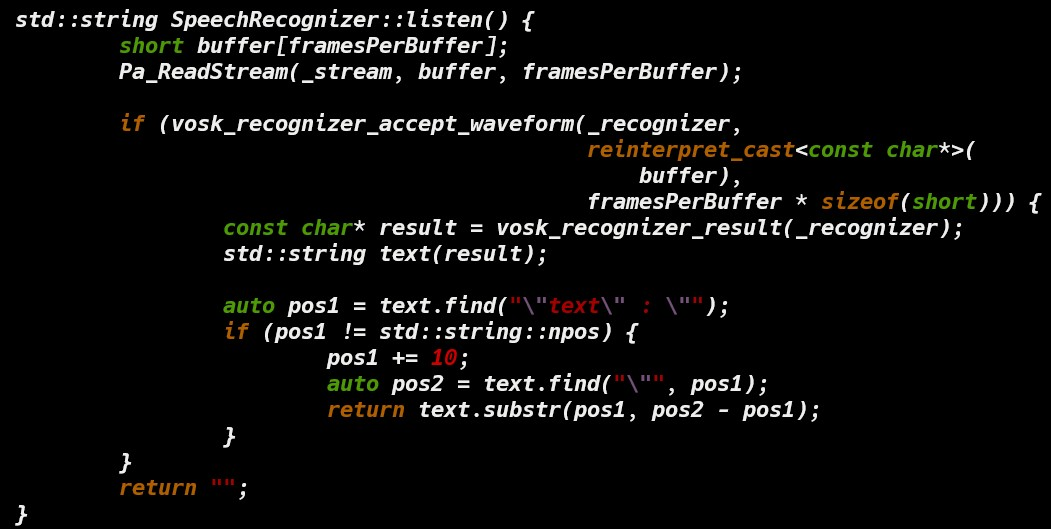
\includegraphics[scale=0.8]{listenSpeechRecognizer.jpg}
	\caption{Метод listen() класса SpeechRecognizer}
\end{figure}

Метод \texttt{SpeechRecognizer::listen()} реализует процесс захвата и обработки аудиоданных для распознавания речи. В начале работы создается буфер размером \texttt{framesPerBuffer} для хранения аудиосэмплов в 16-битном формате (\texttt{short}). С помощью функции \texttt{Pa\_ReadStream} осуществляется чтение аудиопотока из микрофона, при этом данные записываются в подготовленный буфер. Полученные аудиоданные передаются в распознаватель Vosk через функцию \texttt{vosk\_recognizer\_accept\_waveform}, где происходит их преобразование в текстовый формат.

Если распознавание прошло успешно, функция \texttt{vosk\_recognizer\_result} возвращает результат в виде JSON-строки, содержащей распознанный текст. Из этой строки извлекается непосредственно текстовая часть между полями \texttt{\string"text\string" : \string"} и закрывающей кавычкой. Для этого используется поиск позиций соответствующих подстрок и последующее выделение нужного фрагмента. Если текст успешно извлечен, он возвращается как результат работы метода. В случае неудачного распознавания или отсутствия текста в результате возвращается пустая строка.

Таким образом, метод обеспечивает непрерывный цикл захвата аудио, его преобразование в текст и извлечение распознанных фраз из структуры результата, возвращая их для дальнейшей обработки в системе.

\newpage
